\documentclass[12pt,a4paper]{ctexart}

\usepackage{geometry}
\geometry{margin=2.5cm}
\usepackage{graphicx}
\usepackage{hyperref}
\usepackage{setspace}
\usepackage{booktabs}
\usepackage{longtable}
\usepackage{array}
\usepackage{tabularx}
\usepackage{enumitem}
\usepackage{amssymb}
\usepackage{float}
\usepackage{capt-of}

\onehalfspacing
\setlength{\parindent}{2em}
\setlength{\parskip}{0.3em}
\setlist[itemize]{leftmargin=2.5em, itemsep=0.2em}
\setlist[enumerate]{leftmargin=2.8em, itemsep=0.2em}
\renewcommand{\arraystretch}{1.2}
\setcounter{tocdepth}{2}

\newcolumntype{L}[1]{>{\raggedright\arraybackslash}p{#1}}
\newcolumntype{C}[1]{>{\centering\arraybackslash}p{#1}}
\newcolumntype{Y}{>{\raggedright\arraybackslash}X}

\newcommand{\DocumentTitle}{类 Discord 实时社区交流系统技术设计文档}
\newcommand{\DocumentVersion}{V1.1}
\newcommand{\CourseName}{创新创业基础与实践}
\newcommand{\StudentName}{陈瀚钦 \space 范宇扬}
\newcommand{\StudentId}{2023051604062 2023051604100}
\newcommand{\ClassName}{2023级 软件工程3班}
\newcommand{\Instructor}{张扬}

% 模块规格表（用于第 3 章模块分解）
\newcommand{\ModuleSpec}[7]{%
  \par\medskip
  \noindent{\bfseries #1\quad #2}\par
  \vspace{0.25em}
  \noindent\begin{tabularx}{\linewidth}{L{2.8cm}Y}
    \toprule
    覆盖需求 & #3 \\
    主要职责 & #4 \\
    对外契约 & #5 \\
    数据与事件 & #6 \\
    依赖与约束 & #7 \\
    \bottomrule
  \end{tabularx}
  \par\medskip
}

% 实体规格表（用于第 5 章数据设计）
\newcommand{\EntityTable}[6]{%
  \par\medskip
  \noindent{\bfseries #1}\par
  \vspace{0.25em}
  \noindent\begin{tabularx}{\linewidth}{L{2.8cm}Y}
    \toprule
    实体说明 & #2 \\
    关键字段 & #3 \\
    约束 & #4 \\
    关联关系 & #5 \\
    删除或失效规则 & #6 \\
    \bottomrule
  \end{tabularx}
  \par\medskip
}

% 接口规格表（用于第 4 章接口设计）
\newcommand{\CommandSpec}[8]{%
  \par\medskip
  \noindent{\bfseries #1}\par
  \vspace{0.25em}
  \noindent\begin{tabularx}{\linewidth}{L{2.8cm}Y}
    \toprule
    用途 & #2 \\
    输入 & #3 \\
    输出 & #4 \\
    权限要求 & #5 \\
    失败场景 & #6 \\
    触发事件 & #7 \\
    相关实体 & #8 \\
    \bottomrule
  \end{tabularx}
  \par\medskip
}

% 事件规格表（用于第 4 章接口设计的实时事件）
\newcommand{\EventSpec}[6]{%
  \par\medskip
  \noindent{\bfseries #1}\par
  \vspace{0.25em}
  \noindent\begin{tabularx}{\linewidth}{L{2.8cm}Y}
    \toprule
    触发时机 & #2 \\
    事件载荷 & #3 \\
    接收方 & #4 \\
    客户端动作 & #5 \\
    可靠性要求 & #6 \\
    \bottomrule
  \end{tabularx}
  \par\medskip
}

\hypersetup{
  hidelinks,
  pdftitle={\DocumentTitle},
  pdfauthor={\StudentName}
}

\begin{document}

\hypersetup{pageanchor=false}
\begin{titlepage}
  \centering
  \vspace*{3cm}
  {\heiti\zihao{2}\DocumentTitle\par}
  \vspace{1.5cm}
  {\zihao{-3}\DocumentVersion\par}
  \vspace{2cm}
  \begin{tabular}{L{4cm}L{8cm}}
    课程名称： & \CourseName \\
    学生姓名： & \StudentName \\
    学\hspace{1.8em}号： & \StudentId \\
    班\hspace{1.8em}级： & \ClassName \\
    指导教师： & \Instructor \\
    完成日期： & \today \\
  \end{tabular}
  \vfill
  {\zihao{-4}本文档用于描述类 Discord 实时社区交流系统的整体架构、模块设计、接口协议、数据模型及部署方案。\par}
\end{titlepage}

\hypersetup{pageanchor=true}
\pagenumbering{Roman}

\section*{修订记录}
\addcontentsline{toc}{section}{修订记录}
\noindent\begin{tabularx}{\linewidth}{C{2.2cm}C{3cm}C{3cm}Y}
  \toprule
  版本 & 日期 & 修订人 & 修订说明 \\
  \midrule
  V1.0 & 2026年5月24日 & 待填写 & 初始版本，完成类 Discord 实时社区交流系统的软件需求规格说明书。 \\
  V1.1 & 2026年5月24日 & 待填写 & 补充 MVP 范围、优先级、开发追踪、逻辑接口、实时事件、数据约束、权限矩阵和验收映射。 \\
  \bottomrule
\end{tabularx}

\clearpage
\tableofcontents

\clearpage
\pagenumbering{arabic}
\setcounter{page}{1}

\section{引言}

\subsection{编写目的}
本文档用于定义类 Discord 实时社区交流系统的业务范围、功能需求、接口与数据要求、非功能指标以及验收标准，为课程设计、原型开发、测试设计和后续演示提供统一依据。本文档强调需求层面的完整性与可验证性，不直接展开数据库实现、部署脚本或具体技术选型细节。

\subsection{项目背景}
随着在线学习、兴趣社区协作和远程团队沟通需求持续增长，用户需要一种兼具群组交流、即时消息、语音互动和权限管理能力的实时社区平台。类 Discord 实时社区交流系统面向课程设计场景，聚焦“社区 + 频道 + 实时互动”的核心体验，支持用户围绕不同主题组织文本与语音交流。

\subsection{文档范围}
本软件需求规格说明书覆盖以下内容：
\begin{itemize}
  \item 平台账号体系，包括注册、登录、身份认证、密码找回和个人资料维护。
  \item 社交协作能力，包括好友关系、私聊会话、在线状态与通知提醒。
  \item 社区组织能力，包括社区创建、加入、退出、成员管理、文本频道与语音频道。
  \item 权限控制能力，包括角色定义、频道访问限制和操作授权校验。
  \item 支撑上述业务的接口约束、数据实体定义、性能指标和验收条件。
\end{itemize}

本文档明确不包含以下内容：
\begin{itemize}
  \item 真实多人语音媒体流、屏幕共享和直播能力；v1 仅描述语音频道成员状态同步。
  \item 短视频、机器人平台、第三方开放接口市场等扩展生态能力。
  \item 商业化订阅、广告投放、付费会员和独立运营后台系统。
  \item 具体代码实现、底层数据库建模脚本、自动化部署流程和详细测试用例实现。
\end{itemize}

\subsection{预期读者}
本文档的主要读者包括：
\begin{itemize}
  \item 项目开发人员：依据需求拆分模块、设计接口与实现功能。
  \item 项目测试人员：基于功能需求和验收条件制定测试方案。
  \item 任课教师或评审人员：检查系统目标、需求完整性和课程成果质量。
  \item 项目成员：统一业务术语、边界理解和交付预期。
\end{itemize}

\subsection{系统边界}
本系统围绕实时社区交流场景展开，其边界如下：
\begin{itemize}
  \item 系统内部：用户账号、好友关系、社区空间、频道组织、消息发送、语音状态、角色权限、通知提醒。
  \item 系统外部：邮件或短信验证码服务、文件存储服务、推送通知服务、浏览器与客户端运行环境。
  \item 边界规则：凡涉及社区交流主流程的数据生产、分发、展示与访问控制，均属于系统职责；依赖的基础通信或存储能力由外部服务提供。
\end{itemize}

\subsection{术语与缩略语}
\noindent\begin{tabularx}{\textwidth}{L{3cm}Y}
  \toprule
  术语或缩写 & 说明 \\
  \midrule
  社区（Server） & 用户围绕某一主题或组织建立的交流空间，承载频道、成员、角色和权限规则。 \\
  频道（Channel） & 社区内部的交流单元，分为文本频道和语音频道两类。 \\
  文本频道 & 用于发送文字、图片、文件和提及消息的频道。 \\
  语音频道 & 用于实时语音接入、状态同步和在线互动的频道。 \\
  私聊（Direct Message, DM） & 两个用户之间的一对一会话，不依附于某个社区。 \\
  在线状态（Presence） & 用户当前的可用状态，如在线、离开、忙碌、隐身和离线。 \\
  提及（Mention） & 在消息中使用特定标记引用用户，使其收到重点提醒。 \\
  角色（Role） & 社区内可分配给成员的权限集合，用于控制频道访问和管理操作。 \\
  实时同步 & 客户端与服务端通过长连接或事件机制及时传播状态变化的能力。 \\
  SRS & Software Requirements Specification，软件需求规格说明书。 \\
  \bottomrule
\end{tabularx}

\subsection{参考依据}
\begin{itemize}
  \item 软件工程课程设计任务要求与课程文档规范。
  \item 软件需求规格说明书常见写作规范与高校课程报告格式要求。
  \item 即时通信与在线社区平台的通用业务模式和交互需求。
  \item 面向实时系统的性能、安全、可用性与权限控制基本原则。
\end{itemize}

\section{系统架构设计}

\subsection{系统架构图}
\begin{figure}[H]
\centering
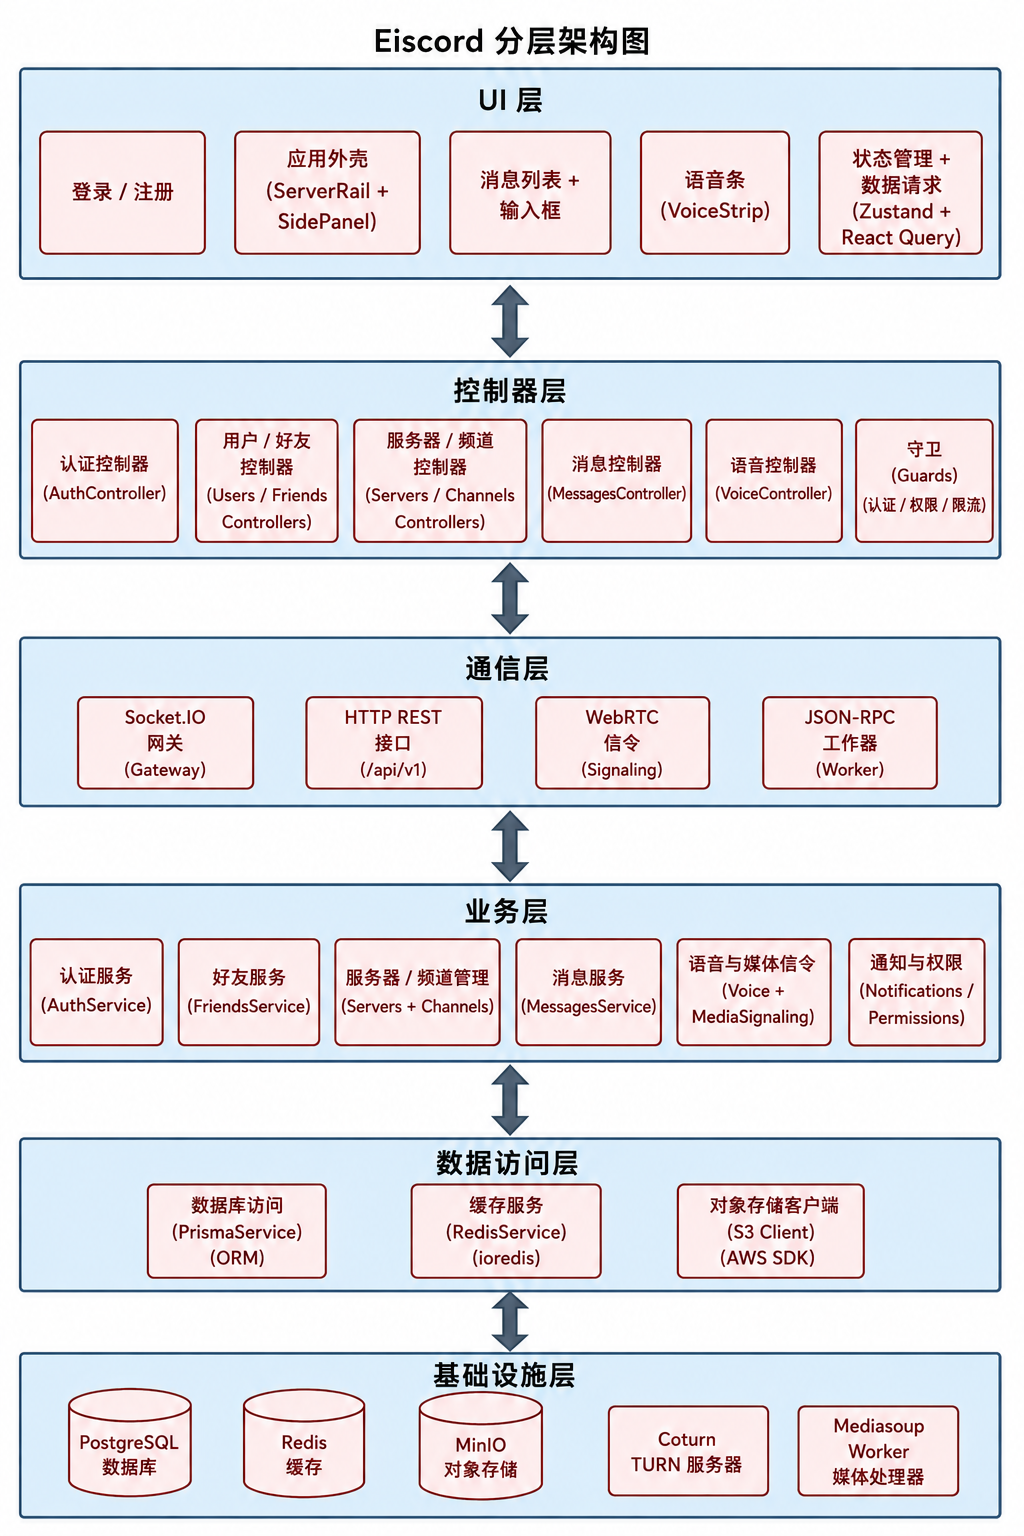
\includegraphics[width=\textwidth]{figures/arch-layers.png}
\caption{系统分层架构图}
\label{fig:architecture}
\end{figure}

\subsection{总体架构设计}
本系统采用前后端分离 + 三层架构设计：

\begin{description}[itemsep=0pt]
  \item[UI 层] React 18 SPA，Vite 构建，react-router-dom 路由，Zustand + React Query 状态管理，Socket.IO 客户端实时通信，mediasoup-client 语音媒体。
  \item[控制器层] NestJS Controllers + Guards（AccessToken / Permission / RateLimit）+ Filters / Interceptors。
  \item[通信层] HTTP REST（Axios）、WebSocket（Socket.IO 4.7）、WebRTC（mediasoup-client）、JSON-RPC（Worker 子进程）。
  \item[业务层] 14 个 NestJS Service 模块，覆盖认证、用户、好友、社区、频道、消息、语音、通知、权限等核心领域。
  \item[数据访问层] Prisma ORM（PostgreSQL）、ioredis（Redis）、AWS S3 SDK（MinIO）。
\end{description}

\subsection{核心模块划分}
\begin{center}
\captionof{table}{核心模块一览}
\begin{tabularx}{\textwidth}{L{2.8cm}L{2.5cm}Y}
\toprule
\textbf{模块} & \textbf{层级} & \textbf{职责} \\
\midrule
Auth 认证 & 业务层 & 注册/登录/JWT 签发/会话管理 \\
Users 用户 & 业务层 & 资料管理、在线状态 \\
Friends 好友 & 业务层 & 好友申请/关系维护/私聊会话 \\
Servers 社区 & 业务层 & 社区 CRUD/角色/成员/邀请 \\
Channels 频道 & 业务层 & 频道 CRUD/权限覆盖 \\
Messages 消息 & 业务层 & 消息发送/分页/已读/去重 \\
Voice 语音 & 业务层 & 语音频道加入/离开/状态同步 \\
MediaSignaling & 业务层 & WebRTC 信令/Mediasoup 编排 \\
Realtime 实时 & 业务+通信层 & Socket.IO 网关/事件广播/房间管理 \\
Notifications 通知 & 业务层 & 通知创建/列表/已读标记 \\
Attachments 附件 & 业务层 & S3 预签名上传/附件生命周期 \\
Permissions 权限 & 业务层 & bitmask 权限计算/校验 \\
Audit 审计 & 业务层 & 关键操作审计日志 \\
Health 健康 & 控制器层 & 服务健康检查 \\
\bottomrule
\end{tabularx}
\end{center}

\subsection{技术选型}
\begin{tabularx}{\textwidth}{L{3.5cm}L{3.5cm}L{4.5cm}}
\toprule
\textbf{层级} & \textbf{选型} & \textbf{版本} \\
\midrule
Web 客户端 & React + TypeScript + Vite & React 18.2 \\
服务端框架 & NestJS & 10.3.8 \\
ORM & Prisma & 5.13.0 \\
主数据库 & PostgreSQL（Docker） & 16 Alpine \\
缓存与状态 & Redis（Docker） & 7 Alpine \\
实时通信 & Socket.IO & 4.7.5 \\
语音媒体 & Mediasoup & 3.15.7 \\
对象存储 & MinIO / AWS S3 SDK & 3.1041.0 \\
TURN 中继 & Coturn & latest \\
数据验证 & Zod & 3.23.8 \\
状态管理 & Zustand + React Query & 4.5.2 / 5.32.1 \\
包管理 & pnpm monorepo & 9.15.4 \\
\bottomrule
\end{tabularx}

\subsection{模块间依赖关系}
\begin{itemize}[itemsep=0pt]
  \item Controller $\to$ Service $\to$ PrismaService（垂直调用）
  \item MessagesService 依赖 NotificationsService、RealtimePublisher
  \item VoiceService / MediaSignalingService 依赖 MediasoupWorkerClient、MediasoupRouterRegistry
  \item FriendsService 依赖 NotificationsService
  \item 权限校验链路：AccessTokenGuard $\to$ PermissionGuard $\to$ RateLimitGuard
  \item 请求链路：RequestIdMiddleware $\to$ ApiExceptionFilter $\to$ ApiResponseInterceptor
\end{itemize}

\section{模块与功能详细设计}

\subsection{模块总览}

系统由 14 个 NestJS 服务端模块 + 1 个 Mediasoup Worker 子进程 + 9 个前端功能模块组成，以下按服务端模块说明核心职责和关键技术实现。

\subsection{核心功能模块设计}

\subsubsection{用户登录模块}

涉及接口：RegisterUser、LoginUser。关键实体：User、AuthSession。

业务流程：
\begin{enumerate}[itemsep=0pt]
  \item 用户提交注册信息（用户名、邮箱、密码），系统校验唯一性和密码强度，写入 users 表
  \item 登录时查询 users 表验证 bcrypt 密码哈希，验证通过后创建 auth\_sessions 行
  \item 返回 access\_token（JWT 短有效期）+ refresh\_token（长有效期），附带用户/好友/社区/未读/通知快照
  \item 刷新令牌时验证旧 refresh\_token 未过期/未撤销，轮换生成新令牌对；登出时设置 revoked\_at
\end{enumerate}

\subsubsection{消息发送模块}

涉及接口：SendMessage、LoadMessages、MarkRead、DeleteMessage。关键实体：Message、ReadState、MessageAttachment、MessageMention。

\textbf{频道消息流程：}
\begin{enumerate}[itemsep=0pt]
  \item 事务内执行：INSERT messages → INSERT message\_attachments → INSERT message\_mentions
  \item 发送者标记已读（markSenderRead），其他频道成员 unread\_count + 1（incrementChannelUnread）
  \item @提及触发通知创建（NotificationsService.createNotification）
  \item 事务提交后广播 MessageCreated + UnreadUpdated 实时事件
\end{enumerate}

\begin{figure}[H]
\centering
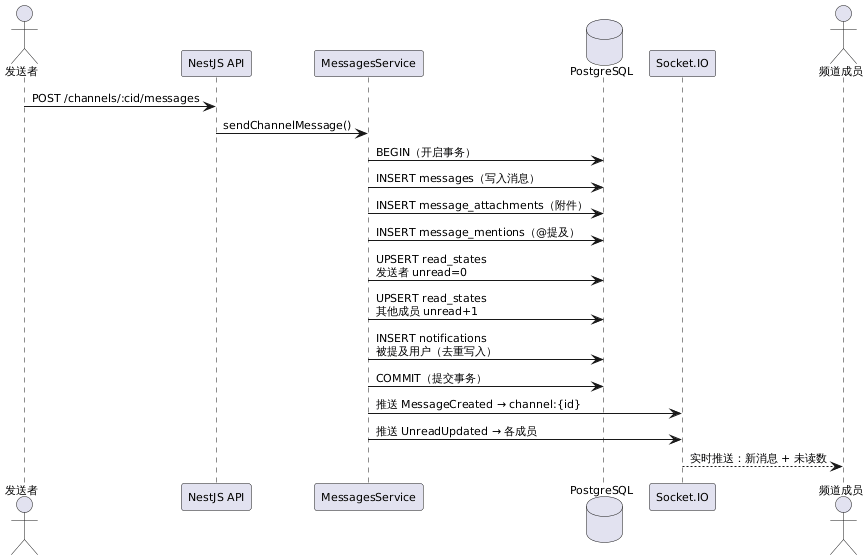
\includegraphics[width=0.80\textwidth]{figures/v1.png}
\caption{频道消息发送事务流程}
\label{fig:msg-channel}
\end{figure}

\textbf{DM 私聊流程：} 同上，区别在于关联 direct\_conversations，仅对接收方 +1 未读，并创建 direct\_message 通知。

\begin{figure}[H]
\centering
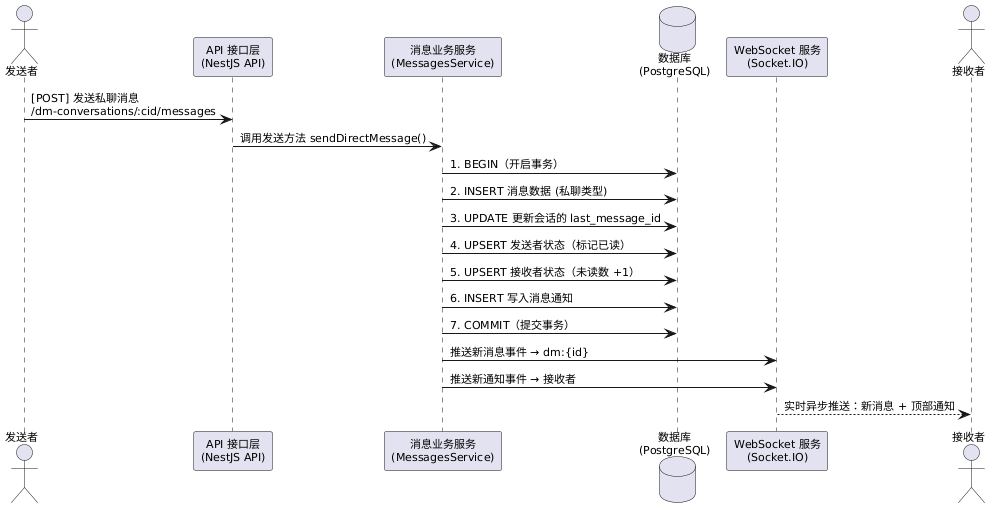
\includegraphics[width=0.75\textwidth]{figures/dmflow.png}
\caption{DM 私聊发送事务流程}
\label{fig:msg-dm}
\end{figure}

\textbf{消息去重机制：} 通过 \texttt{(senderId, channelId/conversationId, clientMessageId)} 唯一约束防重复。发送前先查询已有消息，存在则直接返回。

\textbf{游标分页加载：} 以 (created\_at DESC, id DESC) 排序，返回 pageLimit + 1 条判断是否有下一页，next\_cursor 编码为 base64url。

\subsubsection{语音通信模块}

涉及接口：JoinVoiceChannel、UpdateVoiceState、LeaveVoiceChannel。关键实体：VoiceSession。

\begin{enumerate}[itemsep=0pt]
  \item 用户 POST join → 创建 VoiceSession → MediaSignaling.prepareRouter 获取/创建 Mediasoup Router
  \item 创建 WebRTC Transport（send + recv），返回 ICE/DTLS 参数 + TURN 凭证（HMAC-SHA1 签名）
  \item 客户端创建 mediasoup-client Transport 完成 DTLS 握手，发送方创建 Producer（kind=audio）
  \item 服务端为收听方创建 Consumer，状态变化广播 VoiceStateChanged
  \item 协商超时机制：超出 negotiationDeadline（$\sim$30s）自动清理僵死会话
  \item Mediasoup Worker 崩溃时 RouterRegistry 标记 Router 失效，客户端需重新 join
\end{enumerate}

\begin{figure}[H]
\centering
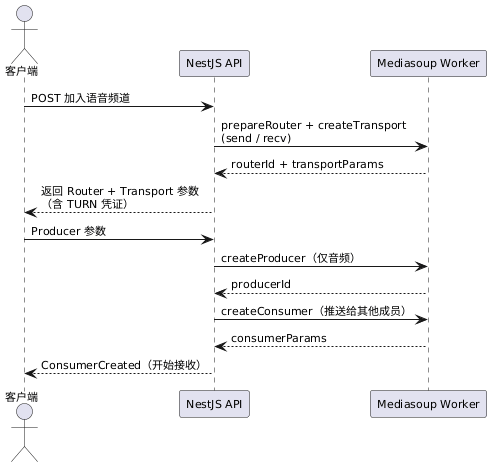
\includegraphics[width=0.78\textwidth]{figures/voice.png}
\caption{WebRTC 语音信令流程}
\label{fig:voice}
\end{figure}

\subsubsection{权限管理模块}

涉及接口：CheckPermission、AssignRole。关键实体：Role、PermissionOverwrite、MembershipRole。

\textbf{权限模型：} bitmask 组合。Owner（全权限）$\to$ 角色权限并集 $\to$ 频道覆盖（allowBits / denyBits）。

权限位定义：
\begin{center}
\begin{tabularx}{\textwidth}{L{3cm}L{3cm}Y}
\toprule
\textbf{权限} & \textbf{位值} & \textbf{说明} \\
\midrule
ViewChannel & 1 & 查看频道 \\
SendMessage & 2 & 发送消息 \\
ManageMessage & 4 & 管理消息（删除）\\
ManageChannel & 8 & 管理频道 \\
JoinVoice & 16 & 加入语音频道 \\
ManageMember & 32 & 管理成员 \\
ManageRole & 64 & 管理角色 \\
CreateInvite & 128 & 创建邀请 \\
ViewAudit & 256 & 查看审计 \\
SpeakVoice & 512 & 语音发言 \\
ListenVoice & 1024 & 收听语音 \\
\bottomrule
\end{tabularx}
\end{center}
默认成员权限 = ViewChannel $|$ SendMessage $|$ JoinVoice $|$ SpeakVoice $|$ ListenVoice（= 1555）。

\subsubsection{实时事件模块}

技术实现：Socket.IO 4.7 网关，房间命名规则：
\begin{itemize}[itemsep=0pt]
  \item \texttt{user:\{id\}} --- 用户私有推送
  \item \texttt{server:\{id\}} --- 社区公告
  \item \texttt{channel:\{id\}} --- 频道公告
  \item \texttt{voice:\{id\}} --- 语音事件
\end{itemize}

核心事件类型（20 种）：MessageCreated, MessageDeleted, UnreadUpdated, NotificationCreated, PresenceChanged, MemberJoined, MemberChanged, ChannelChanged, PermissionChanged, VoiceMemberJoined/Left, VoiceStateChanged, VoiceRouterCapabilities, VoiceTransportCreated/Connect, VoiceProducerCreated, VoiceConsumerCreated/Resumed, VoiceProducerClosed, VoiceActiveSpeaker, SyncState。

断线重连后客户端发送 SyncState 全量同步当前状态。

\subsubsection{前端架构}

采用 React 18 + Vite + TypeScript SPA，9 个功能模块：auth, servers, channels, messages, voice, friends, notifications, permissions, profile。共享组件 17 个（AppShell, ServerRail, MessageList, MessageComposer, VoiceStrip 等）。状态管理使用 Zustand（auth-store, workspace-store, toast-store）+ React Query（服务端数据缓存/失效/重取）。
\section{接口与数据需求}

本章定义系统对外表现出的逻辑接口、实时事件和核心数据实体。接口名称仅表示业务命令或事件契约，不限定 REST、GraphQL、WebSocket、消息队列或数据库实现方式。

\subsection{客户端界面要求}
\noindent\begin{tabularx}{\textwidth}{L{3.2cm}Y}
  \toprule
  界面区域 & 要求说明 \\
  \midrule
  登录与注册界面 & 应清晰区分登录、注册、找回密码入口，表单项完整，错误信息可读，并支持基础输入校验。 \\
  社区导航区 & 应展示用户已加入的社区列表，支持进入社区、创建社区和接受邀请后的快速跳转。 \\
  频道列表区 & 应展示当前社区下的文本频道与语音频道，并按权限过滤用户不可访问的频道。 \\
  消息主面板 & 应支持消息列表滚动、历史加载、输入框发送、附件上传入口、提及提示、撤回和删除反馈。 \\
  成员与状态区 & 应展示当前社区在线成员、离线成员、角色摘要和语音频道内的成员状态变化。 \\
  通知入口 & 应展示未读数量，并允许用户统一查看好友申请、私聊提醒、提及通知和系统提示。 \\
  语音控制区 & 当用户加入语音频道后，应提供静音、闭麦、恢复和离开频道等状态操作入口。 \\
  权限管理区 & 社区所有者或管理员应能维护角色、成员角色分配和频道级权限覆盖规则。 \\
  \bottomrule
\end{tabularx}

\subsection{逻辑命令接口}
逻辑命令表示客户端或系统内部发起的业务动作。所有命令都必须携带可识别的操作者上下文，并在写入核心数据前完成身份与权限校验。

\CommandSpec{RegisterUser}{
创建平台账号和基础用户档案。
}{
\texttt{username}、\texttt{email\_or\_phone}、\texttt{password}、可选验证凭据。
}{
注册结果、\texttt{user\_id}、账号验证状态。
}{
仅访客用户可发起；注册信息必须满足唯一性和密码规则。
}{
用户名或邮箱手机号重复；密码不合规；验证凭据无效；注册服务暂不可用。
}{
可触发 \texttt{NotificationCreated} 和审计记录。
}{
User、AuditLog。
}

\CommandSpec{LoginUser}{
验证登录凭证并创建有效会话。
}{
\texttt{login\_identifier}、\texttt{password}、客户端上下文。
}{
会话标识、用户资料摘要、社区列表、好友摘要、未读与通知摘要。
}{
账号必须存在且处于可登录状态。
}{
账号不存在；密码错误；账号禁用；验证未完成；连续失败触发安全限制。
}{
\texttt{PresenceChanged}、\texttt{UnreadUpdated}。
}{
User、Membership、ReadState、Notification、AuditLog。
}

\CommandSpec{ResetPassword}{
通过受信任验证方式重置账号密码。
}{
\texttt{account\_identifier}、验证凭据、新密码。
}{
重置结果和安全提示。
}{
操作者必须通过账号绑定验证。
}{
验证失败；凭据过期；新密码不合规；账号不存在或不可重置。
}{
\texttt{NotificationCreated}。
}{
User、AuditLog。
}

\CommandSpec{UpdateProfile}{
修改用户公开资料和头像元数据。
}{
\texttt{nickname}、\texttt{avatar\_attachment\_id}、\texttt{bio} 等资料字段。
}{
更新后的用户资料摘要。
}{
用户必须已登录且只能修改自身资料。
}{
字段超长；头像附件不可用；资料格式非法。
}{
\texttt{PresenceChanged}。
}{
User、Attachment、AuditLog。
}

\CommandSpec{UpdatePresence}{
更新用户在线状态或根据连接心跳推导状态。
}{
\texttt{desired\_status}、连接标识、心跳时间。
}{
可见状态和状态更新时间。
}{
用户必须有有效会话；系统可基于连接状态覆盖客户端上报状态。
}{
状态值非法；会话失效；连接上下文不可识别。
}{
\texttt{PresenceChanged}。
}{
User、Membership。
}

\CommandSpec{CreateFriendRequest}{
向目标用户发送好友申请。
}{
\texttt{target\_user\_id} 或可搜索标识、申请附言。
}{
好友申请记录和通知结果。
}{
双方必须为平台注册用户，且尚未存在有效好友关系。
}{
目标不存在；向自己申请；重复申请；目标屏蔽或关系已存在。
}{
\texttt{NotificationCreated}。
}{
Friendship、Notification、AuditLog。
}

\CommandSpec{AcceptFriendRequest}{
处理收到的好友申请。
}{
\texttt{friendship\_id}、处理动作。
}{
好友关系状态和双方好友摘要。
}{
操作者必须是申请接收方；申请必须处于待处理状态。
}{
申请不存在；申请已处理；操作者不是接收方。
}{
\texttt{NotificationCreated}、\texttt{PresenceChanged}。
}{
Friendship、DirectConversation、Notification、AuditLog。
}

\CommandSpec{CreateServer}{
创建社区、默认角色和默认频道。
}{
社区名称、简介、图标附件、初始可见性配置。
}{
社区详情、所有者成员记录、默认角色和默认频道摘要。
}{
用户必须已登录且未超过社区创建限制。
}{
输入非法；创建数量超限；默认结构创建失败。
}{
\texttt{MemberJoined}、\texttt{ChannelChanged}、\texttt{PermissionChanged}。
}{
Server、Membership、Role、Channel、AuditLog。
}

\CommandSpec{JoinServer}{
通过邀请加入社区。
}{
\texttt{invite\_code} 或邀请链接、用户上下文。
}{
成员记录、默认角色、可见频道列表。
}{
用户必须已登录；邀请必须有效；用户不得被社区限制访问。
}{
邀请不存在、过期或达到使用上限；用户已加入；用户被封禁。
}{
\texttt{MemberJoined}、\texttt{UnreadUpdated}。
}{
Invitation、Membership、Server、Role、AuditLog。
}

\CommandSpec{LeaveServer}{
退出社区或由管理者移除成员。
}{
\texttt{server\_id}、目标成员、退出或移除原因。
}{
成员关系失效结果和权限刷新结果。
}{
本人可退出；管理员移除成员需要成员管理权限；社区所有者退出前必须转移所有权。
}{
目标成员不存在；无权移除；所有者未转移所有权。
}{
\texttt{PermissionChanged}、\texttt{MemberChanged}、\texttt{VoiceMemberLeft}。
}{
Membership、Role、VoiceSession、AuditLog。
}

\CommandSpec{ManageMember}{
查看成员列表或执行基础成员管理动作。
}{
\texttt{server\_id}、目标成员、管理动作。
}{
成员列表、成员状态或管理动作结果。
}{
查看需具备社区成员身份；管理动作需具备成员管理权限。
}{
无权操作；目标成员不存在；尝试管理高权限成员。
}{
\texttt{MemberChanged}、\texttt{PermissionChanged}。
}{
Membership、Role、AuditLog。
}

\CommandSpec{CreateChannel}{
创建或配置社区频道。
}{
\texttt{server\_id}、频道名称、频道类型、主题、排序、权限覆盖规则。
}{
频道详情和新的频道列表摘要。
}{
操作者必须拥有频道管理权限。
}{
频道类型非法；名称或排序不合规；权限不足；目标社区不存在。
}{
\texttt{ChannelChanged}、\texttt{PermissionChanged}。
}{
Channel、PermissionOverwrite、Role、AuditLog。
}

\CommandSpec{CheckPermission}{
统一计算用户对资源和操作的有效权限。
}{
操作者、目标资源、操作类型、上下文。
}{
允许或拒绝结果、拒绝原因、可选权限摘要。
}{
所有受控业务命令在执行前必须调用等效权限判断。
}{
上下文不完整；目标资源不存在；权限规则冲突但无法解析。
}{
权限拒绝时写入审计；权限规则变化由 \texttt{PermissionChanged} 同步。
}{
Membership、Role、PermissionOverwrite、Channel、AuditLog。
}

\CommandSpec{SendMessage}{
发送私聊或文本频道消息。
}{
会话或频道标识、文本内容、附件列表、提及列表、客户端临时消息标识。
}{
已持久化消息、附件元数据、分发结果。
}{
发送方必须有会话查看和发言权限。
}{
内容为空或超长；附件非法；无权发送；会话不存在；消息重复提交。
}{
\texttt{MessageCreated}、\texttt{UnreadUpdated}、\texttt{NotificationCreated}。
}{
Message、Attachment、DirectConversation、Channel、ReadState、Notification、AuditLog。
}

\CommandSpec{LoadMessages}{
分页加载私聊或频道历史消息。
}{
会话或频道标识、游标、页大小、方向。
}{
消息列表、下一页游标、最近未读位置。
}{
请求者必须拥有目标会话或频道的查看权限。
}{
无权查看；游标无效；目标会话不存在；请求页大小超过限制。
}{
通常不触发广播事件，可配合 \texttt{UnreadUpdated}。
}{
Message、ReadState、DirectConversation、Channel、Membership。
}

\CommandSpec{MarkRead}{
更新用户在会话或频道中的已读位置。
}{
会话或频道标识、最后已读消息标识。
}{
新的未读计数和读取状态。
}{
用户必须能查看目标会话或频道。
}{
消息不属于目标会话；无权查看；读取位置回退不被允许。
}{
\texttt{UnreadUpdated}。
}{
ReadState、Message、Membership、DirectConversation。
}

\CommandSpec{DeleteMessage}{
撤回或删除消息。
}{
\texttt{message\_id}、操作类型、删除原因。
}{
消息可见状态和审计结果。
}{
发送者可撤回自身消息；管理员删除频道消息需具备消息管理权限。
}{
消息不存在；无权操作；消息已删除；跨会话删除。
}{
\texttt{MessageDeleted}、\texttt{UnreadUpdated}。
}{
Message、Notification、ReadState、AuditLog。
}

\CommandSpec{MarkNotificationRead}{
将通知标记为已读。
}{
通知标识列表或全部已读动作。
}{
已读状态和剩余未读计数。
}{
用户只能处理自己的通知。
}{
通知不存在；通知归属不匹配；重复操作。
}{
\texttt{UnreadUpdated}。
}{
Notification、ReadState。
}

\CommandSpec{AssignRole}{
创建、修改、删除角色或为成员分配角色。
}{
角色配置、目标成员、权限集合、优先级。
}{
角色详情、成员角色映射和权限刷新结果。
}{
操作者必须拥有角色管理权限，且不得授予超出自身能力的权限。
}{
角色不存在；默认角色非法删除；目标成员不存在；越权分配。
}{
\texttt{PermissionChanged}、\texttt{MemberChanged}。
}{
Role、Membership、PermissionOverwrite、AuditLog。
}

\CommandSpec{JoinVoiceChannel}{
加入语音频道状态房间。
}{
\texttt{channel\_id}、连接上下文、初始静音和闭麦状态。
}{
语音会话状态和频道成员状态列表。
}{
用户必须有查看和加入目标语音频道的权限。
}{
频道不存在；频道非语音类型；无权加入；已有其他有效语音会话无法切换。
}{
\texttt{VoiceMemberJoined}、必要时触发 \texttt{VoiceMemberLeft}。
}{
VoiceSession、Channel、Membership、PermissionOverwrite、AuditLog。
}

\CommandSpec{UpdateVoiceState}{
更新语音频道中的成员状态。
}{
\texttt{session\_id}、静音状态、闭麦状态、连接状态。
}{
更新后的语音会话状态。
}{
用户必须处于有效语音会话中。
}{
会话不存在；状态值非法；权限已失效；连接超时。
}{
\texttt{VoiceStateChanged}、\texttt{VoiceMemberLeft}。
}{
VoiceSession、Channel、AuditLog。
}

\subsection{实时事件要求}
实时事件用于客户端状态同步。事件消费者不得仅凭事件载荷绕过权限校验；客户端收到事件后仍应基于本地会话上下文更新可见范围内的界面。

\EventSpec{MessageCreated}{
消息成功持久化并通过权限校验后。
}{
\texttt{message\_id}、会话或频道标识、发送者摘要、内容摘要、附件摘要、提及列表、创建时间。
}{
私聊参与者或有权查看目标频道的在线成员。
}{
插入消息、更新最近会话、刷新未读和通知角标。
}{
消息事件应在正常网络下 1 秒内到达目标客户端；断线客户端重连后通过历史消息补齐。
}

\EventSpec{MessageDeleted}{
消息被发送者撤回或管理员删除后。
}{
\texttt{message\_id}、删除类型、操作者摘要、删除时间。
}{
仍有权查看原会话或频道的相关客户端。
}{
将消息展示为已撤回或移除，必要时刷新未读计数。
}{
删除事件必须幂等，重复接收不得恢复已删除消息。
}

\EventSpec{UnreadUpdated}{
用户未读状态变化后。
}{
目标会话或频道标识、未读数量、最后读取位置。
}{
未读状态所属用户的客户端。
}{
更新私聊、频道和通知入口的未读角标。
}{
未读同步延迟不超过 2 秒；重连后以服务端状态为准。
}

\EventSpec{NotificationCreated}{
系统生成好友申请、提及、私聊新消息或管理结果通知后。
}{
\texttt{notification\_id}、通知类型、来源摘要、预览内容、创建时间。
}{
通知目标用户的客户端。
}{
展示通知入口更新和必要的即时提示。
}{
同一业务事件不得重复生成多条等价通知。
}

\EventSpec{PresenceChanged}{
用户登录、离线、隐身、离开或手动切换状态后。
}{
\texttt{user\_id}、可见状态、更新时间。
}{
目标用户好友、同社区可见成员和本人客户端。
}{
刷新好友列表、成员列表和私聊标题区域状态。
}{
隐身状态对他人按离线展示；断线状态应在超时后自动广播。
}

\EventSpec{MemberJoined}{
用户加入社区或社区创建者成为首位成员后。
}{
\texttt{server\_id}、成员摘要、默认角色、加入时间。
}{
目标社区中有权查看成员列表的在线成员。
}{
刷新成员列表、社区导航和默认未读状态。
}{
事件必须在成员关系成功创建后发出。
}

\EventSpec{MemberChanged}{
成员资料、角色或基础管理状态变化后。
}{
\texttt{server\_id}、成员摘要、变更类型、更新时间。
}{
目标社区中有权查看成员列表或管理界面的在线成员。
}{
刷新成员列表、角色标识和管理反馈。
}{
成员被移除后不得继续接收该社区后续成员事件。
}

\EventSpec{ChannelChanged}{
频道创建、编辑、排序或删除后。
}{
\texttt{server\_id}、频道摘要、变更类型。
}{
对目标频道或频道列表有可见权限的社区成员。
}{
刷新频道列表和当前频道可用状态。
}{
权限变更导致不可见的频道应从客户端列表中移除。
}

\EventSpec{PermissionChanged}{
角色、成员角色或频道权限覆盖变化后。
}{
\texttt{server\_id}、变更范围、受影响资源摘要。
}{
受影响社区成员和管理者客户端。
}{
重新计算可见频道、可用操作和管理入口。
}{
权限事件必须先于或同时于受影响资源的后续业务事件生效。
}

\EventSpec{VoiceMemberJoined}{
用户成功加入语音频道状态房间后。
}{
\texttt{channel\_id}、成员摘要、初始语音状态、加入时间。
}{
同语音频道成员和有权查看该语音频道成员列表的用户。
}{
在语音频道成员列表中加入该成员。
}{
本事件只表示状态加入，不承诺真实音频媒体流已经建立。
}

\EventSpec{VoiceMemberLeft}{
用户主动离开、断线超时或权限失效退出语音频道后。
}{
\texttt{channel\_id}、\texttt{user\_id}、离开原因、离开时间。
}{
同语音频道剩余成员和有权查看该语音频道成员列表的用户。
}{
从语音频道成员列表移除该成员。
}{
离开事件必须幂等，重复接收不得造成成员列表异常。
}

\EventSpec{VoiceStateChanged}{
语音频道成员切换静音、闭麦或连接状态后。
}{
\texttt{session\_id}、\texttt{user\_id}、静音状态、闭麦状态、连接状态、更新时间。
}{
同语音频道成员。
}{
更新成员旁的语音状态标识。
}{
状态变化同步时间不超过 3 秒。
}

\subsection{外部接口要求}
\noindent\begin{tabularx}{\textwidth}{L{3cm}L{3.2cm}Y}
  \toprule
  外部接口 & 主要用途 & 要求说明 \\
  \midrule
  文件存储接口 & 消息附件、头像、社区图标上传与访问 & 应支持文件上传、访问地址返回和访问控制；受保护资源必须与业务权限绑定，禁止未授权用户直接访问。 \\
  邮件或短信验证接口 & 注册验证、密码找回、安全通知 & 应支持验证码或重置链接发送，并保证验证结果与账号绑定关系一致。 \\
  推送通知接口 & 应用外提醒或移动端通知 & v1 可作为增强能力；离线用户通知至少应在系统内生成，外部推送失败不得影响核心消息写入。 \\
  日志与监控接口 & 运行日志、异常告警与审计 & 应记录核心操作、异常事件和权限拒绝信息，支持故障分析与审计追踪。 \\
  \bottomrule
\end{tabularx}

\subsection{核心数据实体定义}
以下实体描述系统主要业务对象的结构边界与关联关系。字段名称仅表达业务含义，不限定数据库列名或类型。

\EntityTable{User}{
表示平台注册用户的基础信息、身份状态和个人资料。
}{
\texttt{user\_id}、\texttt{username}、\texttt{nickname}、\texttt{email\_or\_phone}、\texttt{avatar\_url}、\texttt{bio}、\texttt{account\_status}、\texttt{presence\_status}、\texttt{created\_at}
}{
\texttt{username} 和绑定联系方式应保持平台级唯一；密码不得明文存储；在线状态只能取系统定义值。
}{
与 Friendship、DirectConversation、Membership、Message、VoiceSession、Notification、AuditLog 关联。
}{
账号禁用时保留历史消息和审计信息；账号删除或注销应使登录凭证失效，并按隐私要求处理公开资料展示。
}

\EntityTable{Friendship}{
表示两名用户之间的好友申请和好友关系。
}{
\texttt{friendship\_id}、\texttt{requester\_id}、\texttt{addressee\_id}、\texttt{status}、\texttt{created\_at}、\texttt{updated\_at}
}{
同一对用户同一时间只允许存在一条有效好友关系；状态至少支持待处理、已接受、已拒绝、已删除。
}{
关联两个 User，并驱动 DirectConversation 入口和好友通知。
}{
拒绝或删除后关系不再授予好友能力；历史私聊记录按会话规则保留。
}

\EntityTable{DirectConversation}{
表示两个好友之间的一对一私聊会话。
}{
\texttt{conversation\_id}、参与者用户标识、\texttt{last\_message\_id}、\texttt{created\_at}、\texttt{updated\_at}
}{
同一对用户应复用同一有效私聊会话；会话参与者必须与消息访问权限一致。
}{
关联 User、Friendship、Message、ReadState、Notification。
}{
好友关系删除后可隐藏会话入口，但历史消息仍按隐私和保留策略处理。
}

\EntityTable{Server}{
表示用户创建或加入的社区空间。
}{
\texttt{server\_id}、\texttt{owner\_id}、\texttt{name}、\texttt{icon\_url}、\texttt{description}、\texttt{created\_at}
}{
社区必须有且仅有一个所有者；社区名称在展示层应清晰可识别。
}{
与 Invitation、Channel、Membership、Role、AuditLog 直接关联。
}{
社区删除或归档后，其邀请、频道、成员和语音会话全部失效；历史审计按保留策略保存。
}

\EntityTable{Invitation}{
表示加入社区的邀请凭据。
}{
\texttt{invitation\_id}、\texttt{server\_id}、\texttt{code}、\texttt{created\_by}、\texttt{expires\_at}、\texttt{max\_uses}、\texttt{used\_count}、\texttt{status}
}{
邀请码在有效期内应唯一可解析；使用次数和过期时间必须被校验。
}{
关联 Server、User、Membership。
}{
过期、撤销、达到使用上限或社区失效后不得继续加入。
}

\EntityTable{Membership}{
表示用户加入社区后的成员身份信息。
}{
\texttt{membership\_id}、\texttt{server\_id}、\texttt{user\_id}、\texttt{nick\_in\_server}、\texttt{joined\_at}、\texttt{role\_ids}、\texttt{member\_status}
}{
同一用户在同一社区只允许存在一条有效成员记录；角色集合必须属于同一社区。
}{
连接 User 与 Server，并承载角色分配、成员状态和社区昵称。
}{
退出、移除或封禁后成员权限失效；相关语音会话必须释放。
}

\EntityTable{Channel}{
表示社区内部的文本频道或语音频道。
}{
\texttt{channel\_id}、\texttt{server\_id}、\texttt{name}、\texttt{type}、\texttt{topic}、\texttt{sort\_order}、\texttt{created\_at}
}{
\texttt{type} 至少区分文本频道与语音频道；频道必须隶属于某个社区；排序字段应支持稳定展示。
}{
与 Server、PermissionOverwrite 关联；文本频道关联 Message，语音频道关联 VoiceSession。
}{
频道删除后不再允许发送消息或加入语音状态；历史消息按社区策略保留或隐藏。
}

\EntityTable{Role}{
表示社区内可分配的权限集合。
}{
\texttt{role\_id}、\texttt{server\_id}、\texttt{name}、\texttt{permission\_bits}、\texttt{color}、\texttt{priority}、\texttt{is\_default}
}{
角色必须归属于某个社区；优先级应可比较；默认角色必须始终存在。
}{
与 Server、Membership、PermissionOverwrite 关联，是权限校验的核心依据。
}{
角色删除后应从成员角色集合中移除；默认角色不得被删除到社区无默认权限状态。
}

\EntityTable{PermissionOverwrite}{
表示频道级角色或成员权限覆盖规则。
}{
\texttt{overwrite\_id}、\texttt{channel\_id}、目标角色或成员、允许权限集合、拒绝权限集合。
}{
覆盖规则必须隶属于一个频道；同一频道对同一目标只允许一条有效覆盖规则。
}{
关联 Channel、Role、Membership，并参与 CheckPermission 计算。
}{
频道删除、目标角色删除或目标成员失效后覆盖规则同步失效。
}

\EntityTable{Message}{
表示文本频道或私聊中的消息记录。
}{
\texttt{message\_id}、会话或频道标识、\texttt{sender\_id}、\texttt{content}、\texttt{attachment\_ids}、\texttt{mention\_ids}、\texttt{created\_at}、\texttt{deleted\_at}
}{
消息必须关联合法发送者与会话上下文；删除或撤回后应保留可审计状态字段。
}{
与 User、Channel 或 DirectConversation、Attachment、Notification、ReadState、AuditLog 关联。
}{
撤回或删除后不得以普通消息展示；必要元数据保留用于审计、未读修正和通知回溯。
}

\EntityTable{Attachment}{
表示消息附件、头像和社区图标等文件元数据。
}{
\texttt{attachment\_id}、\texttt{owner\_id}、\texttt{storage\_key}、\texttt{file\_name}、\texttt{mime\_type}、\texttt{size}、\texttt{created\_at}
}{
附件大小和类型必须满足配置限制；访问附件必须结合业务上下文授权。
}{
可关联 User、Server、Message。
}{
所属消息删除或资源替换后，附件可进入不可见或待清理状态；受保护附件不得通过旧地址越权访问。
}

\EntityTable{ReadState}{
表示用户在私聊或频道中的最近读取位置和未读状态。
}{
\texttt{read\_state\_id}、\texttt{user\_id}、会话或频道标识、\texttt{last\_read\_message\_id}、\texttt{unread\_count}、\texttt{updated\_at}
}{
每个用户对每个会话或频道最多保留一条有效读取状态；读取位置不得指向无权查看的消息。
}{
关联 User、Message、DirectConversation 或 Channel。
}{
用户退出社区后该社区频道读取状态不再授予访问能力；会话隐藏时可保留状态用于恢复。
}

\EntityTable{VoiceSession}{
表示用户在语音频道中的在线状态会话。
}{
\texttt{session\_id}、\texttt{channel\_id}、\texttt{user\_id}、\texttt{joined\_at}、\texttt{mute\_state}、\texttt{deafen\_state}、\texttt{connection\_status}
}{
同一用户同一时刻仅允许一个有效语音会话；状态字段仅表示语音频道成员状态，不表示真实媒体流质量。
}{
与 User 和语音类型 Channel 关联，用于驱动成员列表和实时状态广播。
}{
主动离开、断线超时、权限失效或成员退出社区后会话失效。
}

\EntityTable{Notification}{
表示推送给目标用户的提醒记录。
}{
\texttt{notification\_id}、\texttt{user\_id}、\texttt{type}、\texttt{source\_id}、\texttt{content\_preview}、\texttt{is\_read}、\texttt{created\_at}
}{
通知必须可映射到具体触发事件；\texttt{is\_read} 只能由目标用户或系统已读策略更新。
}{
关联目标 User，并可由 Friendship、Message、Server 管理动作等触发。
}{
来源资源失效后通知可保留摘要但不得继续暴露受限内容。
}

\EntityTable{AuditLog}{
表示安全、权限和关键管理动作的审计记录。
}{
\texttt{audit\_id}、操作者、目标资源、动作类型、结果、失败原因、请求标识、\texttt{created\_at}
}{
登录失败、权限拒绝、成员移除、角色变更、消息删除等关键动作必须记录；不得写入明文密码或完整敏感凭证。
}{
可关联 User、Server、Channel、Message、Membership、Role。
}{
审计日志至少保留 180 天；超期归档或删除不得影响业务数据一致性。
}

\section{数据库设计}

\subsection{ER 图}

\begin{figure}[H]
\centering
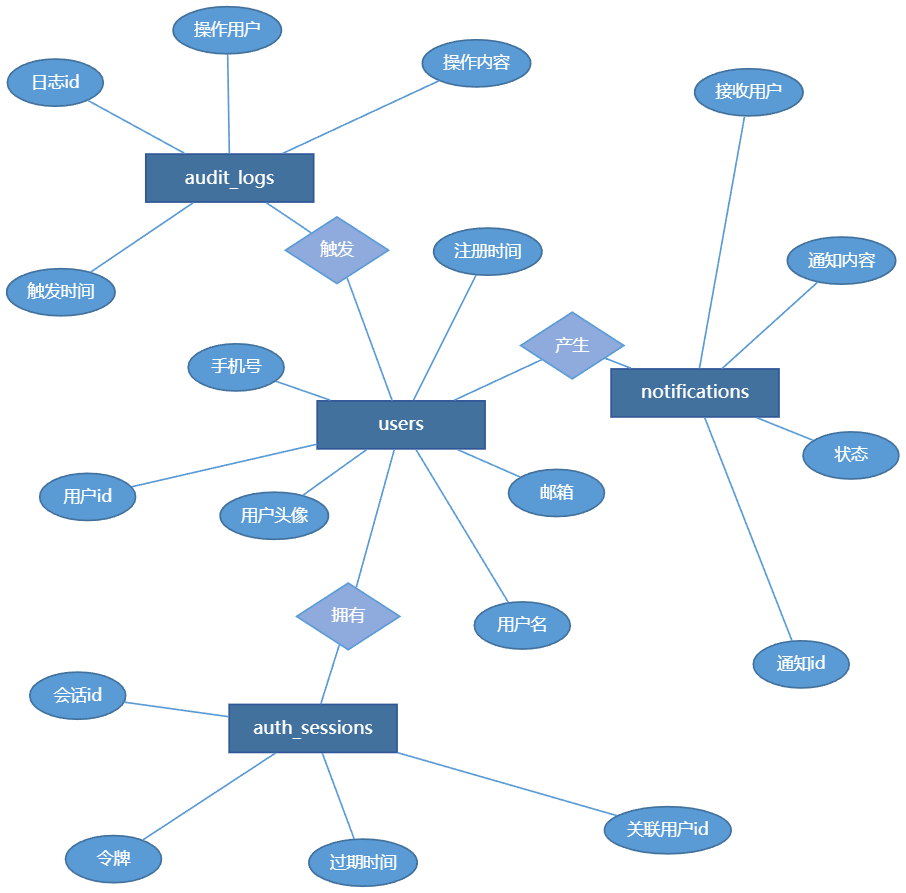
\includegraphics[height=0.45\textheight]{figures/er1.png}
\caption{用户与安全鉴权模块 ER 图}
\label{fig:er-auth}
\end{figure}

\begin{figure}[H]
\centering
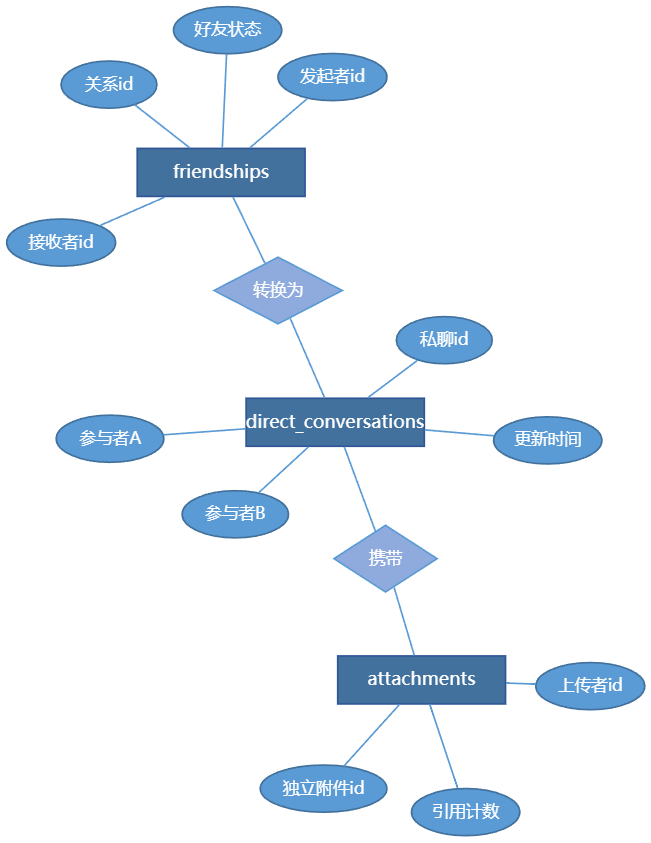
\includegraphics[height=0.40\textheight]{figures/er2.png}
\caption{社交关系与私聊模块 ER 图}
\label{fig:er-social}
\end{figure}

\begin{figure}[H]
\centering
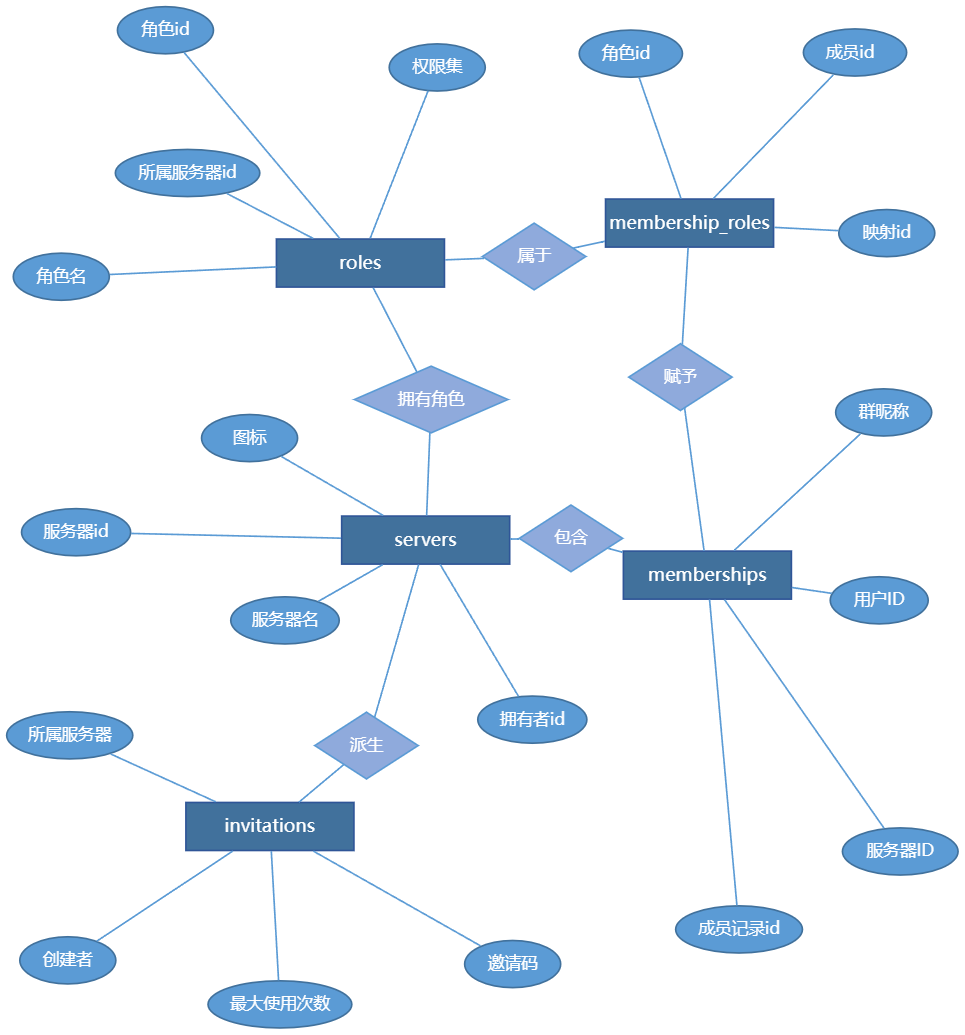
\includegraphics[height=0.45\textheight]{figures/er3.png}
\caption{服务器与成员权限模块 ER 图}
\label{fig:er-server}
\end{figure}

\begin{figure}[H]
\centering
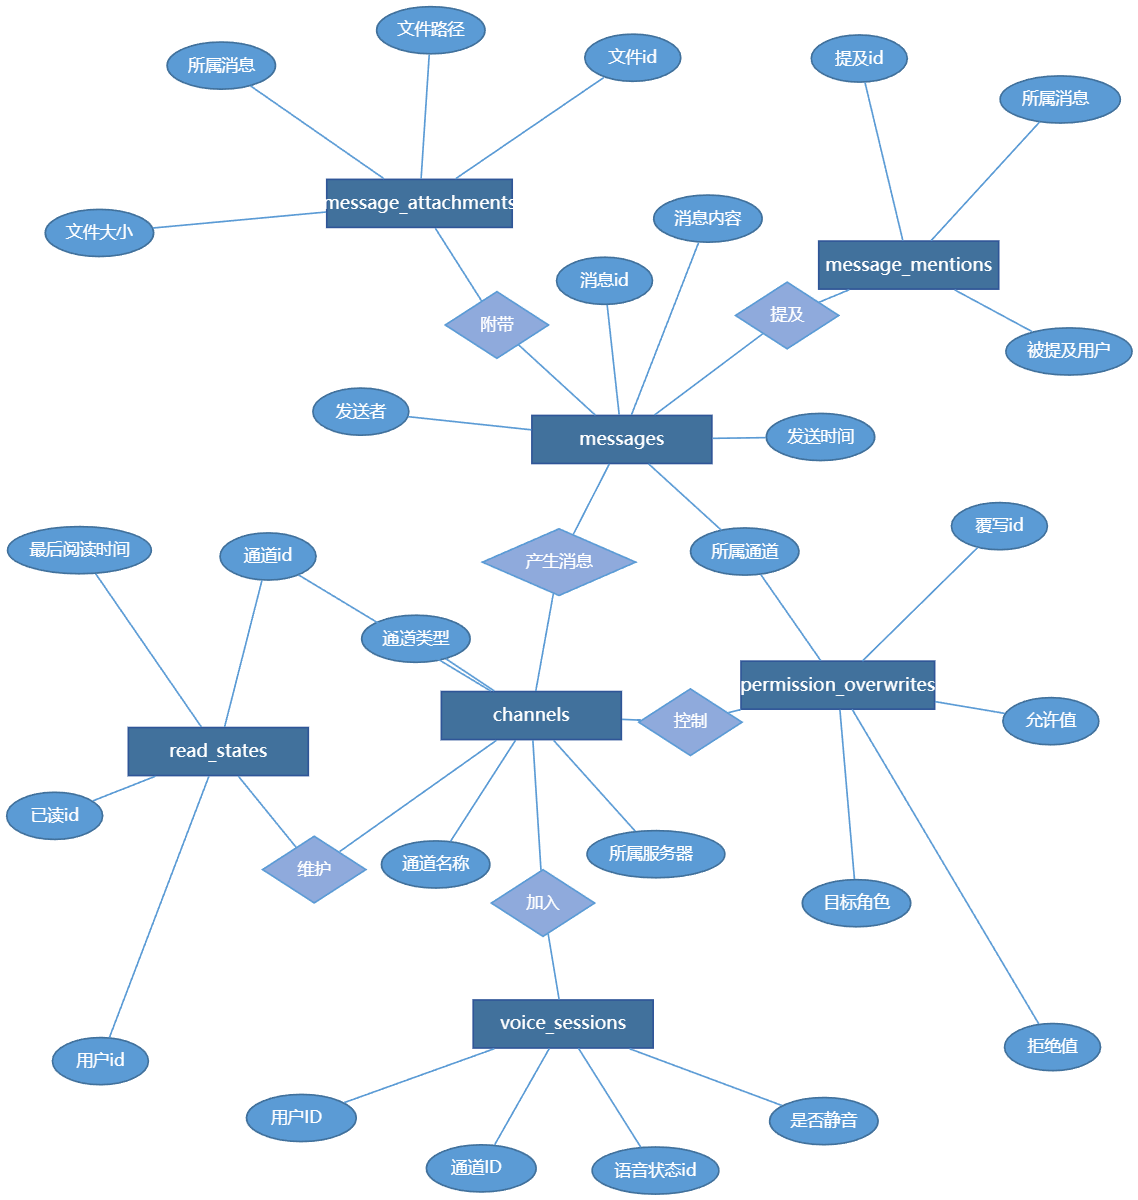
\includegraphics[height=0.50\textheight]{figures/er4.png}
\caption{频道、消息与状态模块 ER 图}
\label{fig:er-channel}
\end{figure}

\subsection{表设计}

系统共 19 个数据模型，以下按业务域分组说明核心实体的关键字段。

\subsubsection{用户与认证}

\noindent\begin{tabularx}{\textwidth}{L{3.2cm}Y}
\toprule
\textbf{表名} & \textbf{关键字段} \\
\midrule
users & id(PK), username(UQ), email\_or\_phone(UQ), password\_hash, nickname, account\_status, presence\_status \\
auth\_sessions & id(PK), user\_id(FK), refresh\_token\_hash(UQ), expires\_at, revoked\_at \\
attachments & id(PK), owner\_id(FK), storage\_key, file\_name, mime\_type, size\_bytes, purpose, status \\
\bottomrule
\end{tabularx}

\subsubsection{社交与好友}

\noindent\begin{tabularx}{\textwidth}{L{3.2cm}Y}
\toprule
\textbf{表名} & \textbf{关键字段} \\
\midrule
friendships & id(PK), requester\_id(FK), addressee\_id(FK), status(pending/accepted/rejected/deleted) \\
direct\_conversations & id(PK), participant\_a\_id(FK), participant\_b\_id(FK), last\_message\_id(FK) \\
notifications & id(PK), user\_id(FK), type, source\_type, source\_id, dedupe\_key(UQ), is\_read \\
\bottomrule
\end{tabularx}

\subsubsection{社区与权限}

\noindent\begin{tabularx}{\textwidth}{L{3.2cm}Y}
\toprule
\textbf{表名} & \textbf{关键字段} \\
\midrule
servers & id(PK), owner\_id(FK), name, icon\_attachment\_id, description, status \\
invitations & id(PK), server\_id(FK), code(UQ), created\_by\_id(FK), expires\_at, max\_uses, used\_count \\
memberships & id(PK), server\_id(FK), user\_id(FK), nick\_in\_server, member\_status \\
roles & id(PK), server\_id(FK), name, permission\_bits(BigInt), color, priority, is\_default \\
membership\_roles & membership\_id(FK), role\_id(FK)（联合主键）\\
permission\_overwrites & id(PK), channel\_id(FK), target\_type, target\_id, allow\_bits, deny\_bits \\
\bottomrule
\end{tabularx}

\subsubsection{频道、消息与语音}

\noindent\begin{tabularx}{\textwidth}{L{3.2cm}Y}
\toprule
\textbf{表名} & \textbf{关键字段} \\
\midrule
channels & id(PK), server\_id(FK), name, type(TEXT$|$VOICE), sort\_order \\
messages & id(PK), scope\_type, channel\_id, conversation\_id, sender\_id(FK), content, visibility, client\_message\_id \\
message\_attachments & message\_id(FK), attachment\_id(FK)（联合 PK）\\
message\_mentions & message\_id(FK), mentioned\_user\_id(FK)（联合 PK）\\
read\_states & id(PK), user\_id(FK), scope\_type, channel\_id, conversation\_id, last\_read\_message\_id, unread\_count \\
voice\_sessions & id(PK), channel\_id(FK), user\_id(FK), mute\_state, deafen\_state, connection\_status, router\_id, producer\_id \\
audit\_logs & id(PK), actor\_id(FK), action, result, target\_type, target\_id, metadata(JSONB) \\
\bottomrule
\end{tabularx}
\section{需求追踪与权限矩阵}

\subsection{权限矩阵}

系统采用基于角色的访问控制（RBAC）模型，权限粒度覆盖服务器级别、频道级别和全局管理级别。

\begin{table}[H]
\centering
\caption{核心权限矩阵（G=全局, S=服务器级, C=频道级）}
\begin{tabularx}{\textwidth}{L{3.2cm}L{1.0cm}Y}
\toprule
\textbf{权限} & \textbf{作用域} & \textbf{说明} \\
\midrule
MANAGE\_SERVER & S & 修改服务器名称、图标、删除服务器 \\
MANAGE\_ROLES & S & 创建/编辑/删除角色、分配权限 \\
MANAGE\_CHANNELS & S & 创建/编辑/删除频道 \\
KICK\_MEMBERS & S & 踢出成员（不含封禁） \\
BAN\_MEMBERS & S & 封禁/解封成员 \\
MANAGE\_MESSAGES & C & 删除频道内任意消息 \\
SEND\_MESSAGES & C & 在频道内发送消息 \\
READ\_MESSAGES & C & 查看频道消息历史 \\
CONNECT & C & 加入语音频道 \\
SPEAK & C & 在语音频道内发言 \\
MUTE\_MEMBERS & C & 语音频道内禁言他人 \\
ADMINISTRATOR & G & 拥有所有权限（最高权限） \\
\bottomrule
\end{tabularx}
\label{tab:perm-matrix}
\end{table}

权限继承规则：
\begin{enumerate}[itemsep=0pt]
  \item 服务器所有者拥有所有权限，且不可被撤销。
  \item 成员权限 = 各角色权限的并集（OR 逻辑）。
  \item 频道权限可覆盖服务器级权限：若某频道显式拒绝了成员某权限，则该权限在该频道中无效。
  \item ADMINISTRATOR 权限具有最高优先级，授予即拥有所有权限。
\end{enumerate}

\subsection{需求追踪矩阵}

下表建立功能需求（源自 SRS V1.1）与设计章节之间的双向追溯关系。

\begin{longtable}{L{1cm}L{2.5cm}L{2.5cm}L{2.5cm}L{2.5cm}}
\caption{需求追踪矩阵} \label{tab:trace-matrix} \\
\toprule
\textbf{编号} & \textbf{需求简述} & \textbf{对应模块} & \textbf{对应接口} & \textbf{对应数据库} \\
\midrule
\endfirsthead
\multicolumn{5}{c}{\small（续表）} \\
\toprule
\textbf{编号} & \textbf{需求简述} & \textbf{对应模块} & \textbf{对应接口} & \textbf{对应数据库} \\
\midrule
\endhead
\bottomrule
\endfoot
FR-01 & 用户注册与登录 & Auth 模块（\S 3.2.1） & POST /auth/register, POST /auth/login & users, auth\_sessions \\
FR-02 & JWT 令牌刷新与会话管理 & Auth 模块（\S 3.2.1） & POST /auth/refresh, POST /auth/logout & auth\_sessions \\
FR-03 & 好友添加/删除/搜索 & Users 模块（\S 3.2.2） & POST /friends, GET /friends & friends, friend\_requests \\
FR-04 & 创建/管理社区服务器 & Servers 模块（\S 3.2.3） & POST /servers, PATCH /servers/:id & servers, server\_members \\
FR-05 & 角色与权限分配 & Permissions 模块（\S 3.2.4） & POST /servers/:id/roles, PUT /servers/:id/members/:uid/roles & roles, role\_permissions, member\_roles \\
FR-06 & 文本频道消息收发 & Messages 模块（\S 3.2.5） & POST /channels/:cid/messages, WS MessageCreated & messages, message\_attachments, message\_mentions \\
FR-07 & 未读计数与阅读状态 & Messages 模块（\S 3.2.5） & WS UnreadUpdated & read\_states \\
FR-08 & 语音频道连接与发言 & Voice 模块（\S 3.2.6） & Mediasoup Worker RPC & voice\_sessions \\
FR-09 & 实时通知推送 & Notifications 模块（\S 3.2.7） & WS NotificationCreated & notifications \\
FR-10 & 文件上传（图片/附件） & Media 模块（\S 3.2.8） & POST /files/upload & file\_objects \\
FR-11 & 消息搜索 & Messages 模块（\S 3.2.5） & GET /channels/:cid/messages/search & messages（全文索引） \\
FR-12 & 用户在线状态同步 & Users 模块（\S 3.2.2） & WS PresenceUpdate & —（Redis） \\
FR-13 & 速率限制与防滥用 & Common Guards（\S 3.2.9） & ThrottlerGuard（全局） & — \\
FR-14 & WebSocket 连接认证 & Gateway（\S 3.2.10） & WS connection\_authenticated & auth\_sessions \\
FR-15 & 暗色/亮色主题切换 & Web 前端（\S 8.3） & — & user\_settings \\
\bottomrule
\end{longtable}

每条需求至少对应一个模块定义、一个接口契约和一张数据表，确保设计无遗漏。

\section{非功能需求}

\subsection{性能与容量要求}
\noindent\begin{tabularx}{\textwidth}{L{2cm}L{4.8cm}Y}
  \toprule
  编号 & 指标项 & 目标要求 \\
  \midrule
  NFR-01 & 普通文本消息端到端到达时间 & 在网络正常条件下，文本消息从发送到目标用户可见的时间不超过 1 秒。 \\
  NFR-02 & 语音频道加入与状态同步响应 & 用户加入语音频道以及静音、取消静音等状态变化完成同步的时间不超过 3 秒。 \\
  NFR-03 & 平台容量基线 & 系统应支持不少于 10000 名注册用户、1000 名并发在线用户，以及单社区 5000 名成员规模。 \\
  NFR-04 & 未读与通知同步延迟 & 私聊未读数、提及提醒和通知角标在事件发生后的 2 秒内完成同步。 \\
  \bottomrule
\end{tabularx}

\subsection{可用性与可靠性要求}
\noindent\begin{tabularx}{\textwidth}{L{2cm}L{4.8cm}Y}
  \toprule
  编号 & 指标项 & 目标要求 \\
  \midrule
  NFR-05 & 系统可用性 & 在统计周期内，系统整体可用性不低于 99.5\%。 \\
  NFR-06 & 数据恢复能力 & 关键业务数据应至少每日执行一次备份，发生严重故障后 4 小时内具备恢复核心服务的能力。 \\
  NFR-07 & 异常降级处理 & 当附件服务、通知服务等外部接口异常时，系统核心登录、文本交流和社区浏览能力仍应保持可用。 \\
  \bottomrule
\end{tabularx}

\subsection{安全与隐私要求}
\noindent\begin{tabularx}{\textwidth}{L{2cm}L{4.8cm}Y}
  \toprule
  编号 & 指标项 & 目标要求 \\
  \midrule
  NFR-08 & 传输安全 & 所有账号凭证、消息访问和附件访问请求均应通过加密传输通道完成。 \\
  NFR-09 & 密码与身份凭证保护 & 密码必须以不可逆方式存储，任何接口和日志中均不得输出明文密码或完整敏感凭证。 \\
  NFR-10 & 最小权限访问 & 所有消息、附件、频道访问请求都必须通过角色或成员权限校验，禁止越权读取或操作。 \\
  NFR-11 & 隐私数据最小暴露 & 非好友或无权限成员不得查看不应公开的个人资料、私聊内容和受限频道内容。 \\
  NFR-12 & 安全审计留痕 & 登录失败、权限拒绝、成员移除、消息删除等关键动作必须产生日志，且日志保留不少于 180 天。 \\
  \bottomrule
\end{tabularx}

\subsection{可维护性与可扩展性要求}
\noindent\begin{tabularx}{\textwidth}{L{2cm}L{4.8cm}Y}
  \toprule
  编号 & 指标项 & 目标要求 \\
  \midrule
  NFR-13 & 模块职责清晰性 & 账号、社区、消息、语音、通知和权限等核心模块应具备清晰边界，不允许出现跨模块直接篡改关键数据的实现方式。 \\
  NFR-14 & 关键链路可观测性 & 所有核心业务请求均应具备可追踪标识，使开发或运维人员能够在 5 分钟内通过日志定位一次失败请求。 \\
  NFR-15 & 接口扩展兼容性 & 实时事件和服务端接口在新增字段时不得破坏现有必填字段语义，至少兼容当前主版本客户端。 \\
  NFR-16 & 配置可调整性 & 文件上传限制、通知开关、社区成员上限等关键参数应支持配置化管理，且配置变更在 5 分钟内生效。 \\
  \bottomrule
\end{tabularx}

\subsection{易用性与兼容性要求}
\noindent\begin{tabularx}{\textwidth}{L{2cm}L{4.8cm}Y}
  \toprule
  编号 & 指标项 & 目标要求 \\
  \midrule
  NFR-17 & 多端界面适配 & 系统应至少适配宽度不低于 360 像素的移动端视图和主流桌面端视图，核心功能入口不得缺失。 \\
  NFR-18 & 主流浏览器兼容性 & Web 客户端应支持当前主流版本的 Chrome、Edge、Firefox 和 Safari，核心页面功能表现一致。 \\
  NFR-19 & 操作可理解性 & 用户完成“注册登录、加入社区、发送消息、加入语音频道”四类核心任务时，单项任务的主要操作路径不应超过 3 次关键点击。 \\
  \bottomrule
\end{tabularx}

\section{验收标准}

\subsection{文档验收条件}

本文档的验收需满足以下条件：

\begin{enumerate}[itemsep=0pt]
  \item \textbf{完整性}：文档覆盖全部 8 章内容，无缺失章节或 TODO 占位符。
  \item \textbf{一致性}：章节间交叉引用（如需求追溯矩阵中的模块引用）与对应章节内容一致。
  \item \textbf{可读性}：图表清晰可读，表格排版整齐，代码/接口示例格式规范，无编译警告（Overfull/Underfull hbox 除外）。
  \item \textbf{可追溯性}：第 6 章需求追踪矩阵建立 SRS 功能需求与本 SDD 设计章节的双向追溯。
  \item \textbf{版本标识}：封面、页眉/页脚体现文档版本号 V1.1 和日期。
\end{enumerate}

\subsection{功能场景验收}

以下功能场景作为文档设计的验证依据：

\begin{table}[H]
\centering
\caption{功能场景验收清单}
\begin{tabularx}{\textwidth}{L{1.0cm}L{3.0cm}L{2.5cm}Y}
\toprule
\textbf{编号} & \textbf{场景} & \textbf{涉及模块} & \textbf{验收要点} \\
\midrule
AC-01 & 新用户注册并登录 & Auth & 密码 bcrypt 哈希、JWT 签发、会话写入 auth\_sessions \\
AC-02 & Token 过期后自动刷新 & Auth & Refresh Token 轮换、旧 Token 失效 \\
AC-03 & 搜索用户并发送好友请求 & Users & 好友请求创建、通知推送、接受/拒绝流程 \\
AC-04 & 创建服务器并分配角色 & Servers, Permissions & 服务器创建、默认角色创建、权限继承校验 \\
AC-05 & 频道内发送消息 & Messages & 事务写入、附件和 @提及同步、未读计数更新 \\
AC-06 & 多成员频道消息实时推送 & Messages, Socket.IO & 频道房间广播、未读数事件个性化推送 \\
AC-07 & 加入语音频道并发言 & Voice & Mediasoup Worker 分配、Producer/Consumer 创建 \\
AC-08 & 上传图片作为消息附件 & Media, MinIO & 分片上传、FileObject 记录创建、下载 URL 生成 \\
AC-09 & 服务器所有者删除服务器 & Servers & 级联删除成员/频道/消息/角色（Prisma 级联） \\
AC-10 & 管理员封禁成员 & Servers & 封禁记录创建、成员关系删除、被封禁者即时踢出 \\
\bottomrule
\end{tabularx}
\label{tab:accept-scenarios}
\end{table}

\subsection{异常场景验收}

\begin{table}[H]
\centering
\caption{异常场景验收清单}
\begin{tabularx}{\textwidth}{L{1.0cm}L{3.0cm}L{2.0cm}Y}
\toprule
\textbf{编号} & \textbf{异常场景} & \textbf{期望行为} & \textbf{对应设计} \\
\midrule
EX-01 & 未登录访问受保护 API & 返回 401，含标准错误体 & AccessTokenGuard（\S 3.2.1） \\
EX-02 & 发送消息至无权限的频道 & 返回 403，消息不入库 & PermissionGuard（\S 3.2.4） \\
EX-03 & 超过速率限制 & 返回 429，Retry-After 头 & ThrottlerGuard（\S 3.2.9） \\
EX-04 & 上传超过大小限制的文件 & 返回 413，前端预先校验 & FileSizeValidator（\S 3.2.8） \\
EX-05 & WebSocket 断连 & 客户端自动重连，5次指数退避 & Socket.IO retry（\S 4.2） \\
EX-06 & Redis 不可用 & 在线状态回退数据库，其余功能正常 & Redis health check（\S 2.5） \\
EX-07 & 数据库主键冲突（并发注册） & 返回 409 Conflict，提示用户名已存在 & Prisma unique constraint（\S 5.2） \\
EX-08 & Mediasoup Worker 崩溃 & 自动重启 Worker，语音频道暂时不可用 & Worker 管理（\S 3.2.6） \\
\bottomrule
\end{tabularx}
\label{tab:accept-exceptions}
\end{table}

\subsection{非功能验收}

\begin{enumerate}[itemsep=0pt]
  \item \textbf{性能验收}：在单节点环境下，使用 K6 脚本（见 \texttt{scripts/k6/}）跑基准负载测试，核心 API P95 延迟 $\le$ 200ms，WebSocket 事件投递 P95 $\le$ 100ms。
  \item \textbf{安全验收}：通过 ESLint Security 规则检查；所有密码 bcrypt 哈希验证；JWT 签名使用 RS256 算法；文件上传类型白名单校验；无明文密码出现在日志中。
  \item \textbf{可靠性验收}：Docker Compose down/up 后服务在 30 秒内恢复可用；消息发送在数据库事务失败时自动回滚，不产生脏数据。
  \item \textbf{兼容性验收}：在 Chrome/Firefox/Edge 最新两个主版本上通过全部 E2E 测试（Playwright）。
\end{enumerate}

\subsection{质量检查要求}

\begin{table}[H]
\centering
\caption{质量检查项}
\begin{tabularx}{\textwidth}{L{3.0cm}L{2.5cm}L{2.0cm}Y}
\toprule
\textbf{检查项} & \textbf{工具/方法} & \textbf{频率} & \textbf{通过标准} \\
\midrule
代码规范检查 & ESLint + Prettier & 每次提交 & 零 Error，警告可记录 \\
类型检查 & TypeScript \texttt{tsc --noEmit} & 每次提交 & 零类型错误 \\
单元测试 & Jest（API） & 每次 PR & 覆盖率 $\ge$ 70\%，关键模块 100\% \\
E2E 测试 & Playwright（Web） & 每次 PR & 全部用例通过 \\
API 契约测试 & Jest + SuperTest & 每次 PR & 所有端点响应码与 Schema 匹配 \\
数据库迁移测试 & Prisma Migrate（dry-run） & 每次 PR & 迁移脚本 0 冲突，可逆回滚标记 \\
集成测试 & Jest + Testcontainers（可选） & 每次 PR & 核心流程（注册→发消息→通知）通过 \\
\bottomrule
\end{tabularx}
\label{tab:quality}
\end{table}

本设计文档的所有设计决策均需通过上述验收标准的检验，方可进入下一阶段（编码实现与测试）。


\end{document}
